\section{Wyżarzacz kwantowy}
\begin{frame}
\frametitle{Wyżarzacz kwantowy D-Wave
 }


\begin{itemize}
\item metaheurystyka do znajdowania globalnego minimum 
\item tunelowanie kwantowe (wyjście z minimum lokalnego)
\end{itemize}

\begin{figure}
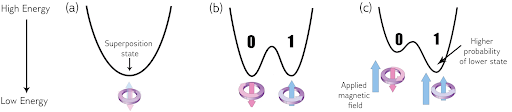
\includegraphics[scale=0.4]{img/18/gorki.png}
\caption{Zmiany energii podczas kwantowego wyżarzania\\source: \url{https://docs.dwavesys.com/docs/latest/c_gs_2.html}}
\end{figure}

\end{frame}
\begin{frame}{Notacja Diraca, iloczyn tensorowy}
  $$\ket{0}=\begin{bmatrix}1\\0
        \end{bmatrix}
        \ket{1}=\begin{bmatrix}0\\1
        \end{bmatrix}$$ 
       $$\ket{00}=\begin{bmatrix}1\\0\\0\\0
       \end{bmatrix}
        \ket{01}=\begin{bmatrix}0\\1\\0\\0
        \end{bmatrix}
        \ket{10}=\begin{bmatrix}0\\0\\1\\0
        \end{bmatrix}
       \ket{11}=\begin{bmatrix}0\\0\\0\\1
       \end{bmatrix}$$ 
        $$\ket{01}=\ket{0}\otimes\ket{1}=
        \begin{bmatrix}1\\0
        \end{bmatrix}\otimes
\begin{bmatrix}0\\1
        \end{bmatrix}=
       \begin{bmatrix}1\cdot0\\1\cdot1\\0\cdot0\\0\cdot1
        \end{bmatrix}=\begin{bmatrix}0\\1\\0\\0
        \end{bmatrix}$$
        
\end{frame}
\begin{frame}{Kwantowy Hamiltonian dla MaxCut}
Funkcja kosztu:
    \begin{itemize}
        \item[] $g(x_1, x_2)=x_1+x_2-2x_1 x_2$, $x_1,x_2 \in\{0,1\}$
        \item[] $x\rightarrow \frac{1}{2}(1-z)$  
        \item[] $g(z_1,z_2)=\frac{1}{2}(1-z_1z_2)$ $z_1,z_2 \in\{-1,1\}$
        \item[]
        $\sigma_z=\begin{pmatrix}  
    1 &0\\
    0 & -1\\
    \end{pmatrix}$
        \item[] $\sigma_z\ket{0}=\ket{0}, \lambda=1$
       \item[] $\sigma_z\ket{1}=-\ket{1}, \lambda=-1$
       \item[] aby zbudować Hamiltonian: $z\rightarrow \sigma_z$
        \item[] $H_{i,j}=\frac{1}{2}(I-{\sigma_z}^i\otimes {\sigma_z}^j)=\begin{pmatrix}  
    0 &0&0&0\\
     0 &1&0&0\\
      0 &0&1&0\\
       0 &0&0&0
    \end{pmatrix} \begin{matrix}
    \ket{00}\\
     \ket{01}\\
      \ket{10}\\
       \ket{11}\\
    \end{matrix}$
        \item[]Wartości włąsne
        \begin{itemize}
            \item $0$ dla $\ket{00}$ i $\ket{11}$ ; $g(00)=0$ $g(11)=0$
             \item $1$ dla $\ket{01}$ i $\ket{10}$ ; $g(01)=1$ $g(10)=1$
        \end{itemize}
    \end{itemize}
    \\
    \small{source: https://grove-docs.readthedocs.io/en/latest/qaoa.html}
\end{frame}
\begin{frame}
\frametitle{Quantum Annealing}
\small
%\begin{columns}[t] % The "c" option specifies centered vertical alignment while the "t" option is used for top vertical alignment
%\column{.5\textwidth} % Left column and width
\begin{itemize}
\item 
startuje w stanie o najniższej energii początkowego H
\item powoli zmienia początkowy H w H dla naszego problemu
\item zmiana dokonuje sie poprzez wprowadzenie  tzw  couplers (J) oraz biases (h) 
\item w idealnej sytuacji system pozostaje w stanie o minimalnej energii przez cały ten proces 
 
 \item działanie kończy się, gdy system znajduje się w stanie o minimalnej energii dla naszego problemu
\item wynik zwracany jest jako klasyczna wartość
\end{itemize}


$$\underbrace{- \frac{A({s})}{2} \left(\sum_i {\sigma_{x}^{(i)}}\right)}_\text{Initial Hamiltonian} + \underbrace{\frac{B({s})}{2} \left(\sum_{i} h_i {\sigma_{z}^{(i)}} + \sum_{i>j} J_{i,j} {\sigma_{z}^{(i)}} {\sigma_{z}^{(j)}}\right)}_\text{Final Hamiltonian}$$

\end{frame}
\begin{frame}{Co należy zrobić?}
 \begin{itemize}
     \item sformułuj problem jako QUBO
\item dopasuj QUBO do architektury komputera
\item otrzymaj rezultaty 
\item dokonaj odwrotnego dopasowania wyników do początkowego QUBO
 \end{itemize}   
\end{frame}

\begin{frame}{QUBO i Hamiltonian}
\begin{block}{QUBO - quadratic and uncontraint cost function $f(x)=x^TQx$}
$f(x)=x^TCx+P\underbrace{(Ax-b)^T(Ax-b)}_{\substack{\text{instead of solving } Ax=b \\ \text{we minimize inner product of }
Ax-b
}}$ 
\end{block}
   $x_i \rightarrow \frac{I-{\sigma_z}^i}{2}$ \arrowupdown  ${\sigma_z}^i= I\otimes I\dots\otimes\underbrace{\sigma_z}_{\text{i- th position}}\dots\otimes I$\\
  
\begin{block}{Hamiltonian}
$H=\sum_{i}c_i\frac{I-{\sigma_z}^i}{2}+P\sum_j (\sum_ia_{j,i}(I-\frac{{\sigma_z}^i}{2})-b_iI)^2$
\end{block} 
Obydwie formy mogą być wejsciem do wyżarzacza kwantowego
\end{frame}

\begin{frame}{Minor Embedding}
 \begin{columns}[t] % The "c" option specifies centered vertical alignment while the "t" option is used for top vertical alignment
\column{.7\textwidth} 
\begin{itemize}
    \item Architektura kwantowego wyżarzacza nie jest grafem pełnym
    
\item konieczna jest transformacja grafu naszego problemu do tej architektury 
\item  zwykle konieczne jest reprezentowanie jednej zmiennej problemu przez wiele qbitów (łańcuchy)

\end{itemize}
\column{.3\textwidth} 
    \begin{figure}[H]
    \centering
    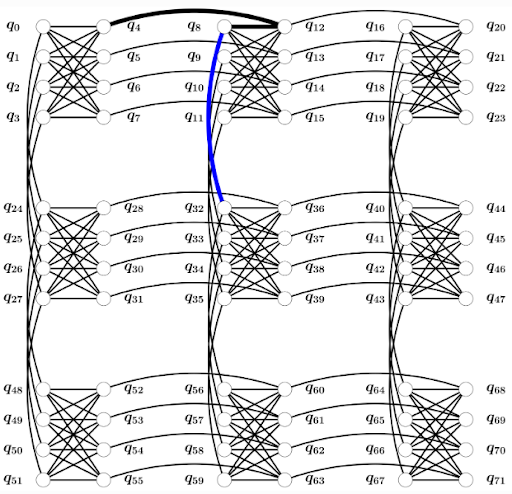
\includegraphics[width=\linewidth]{img/18/chimera.png}
\end{figure}

\end{columns}
 \begin{figure}[H]
    \centering
    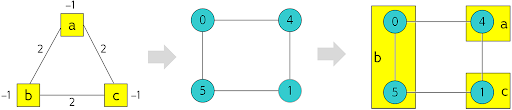
\includegraphics[width=0.9\linewidth]{img/18/simple_embed.png}
\end{figure} 
\tiny Source: https://docs.dwavesys.com/docs/latest/c\_gs\_7.html

\end{frame}
\begin{frame}{Embedowanie pełnego grafu}
\begin{itemize}
    \item przykład jak osadzić graf $K_9$ w grafie Chimera $2\times2$
\item trzy qbity na jedną zmienną  (poza 8)
\item ta metoda działa dla grafów do 9 wierzchołków

\end{itemize}    
\begin{figure}[H]
    \centering
    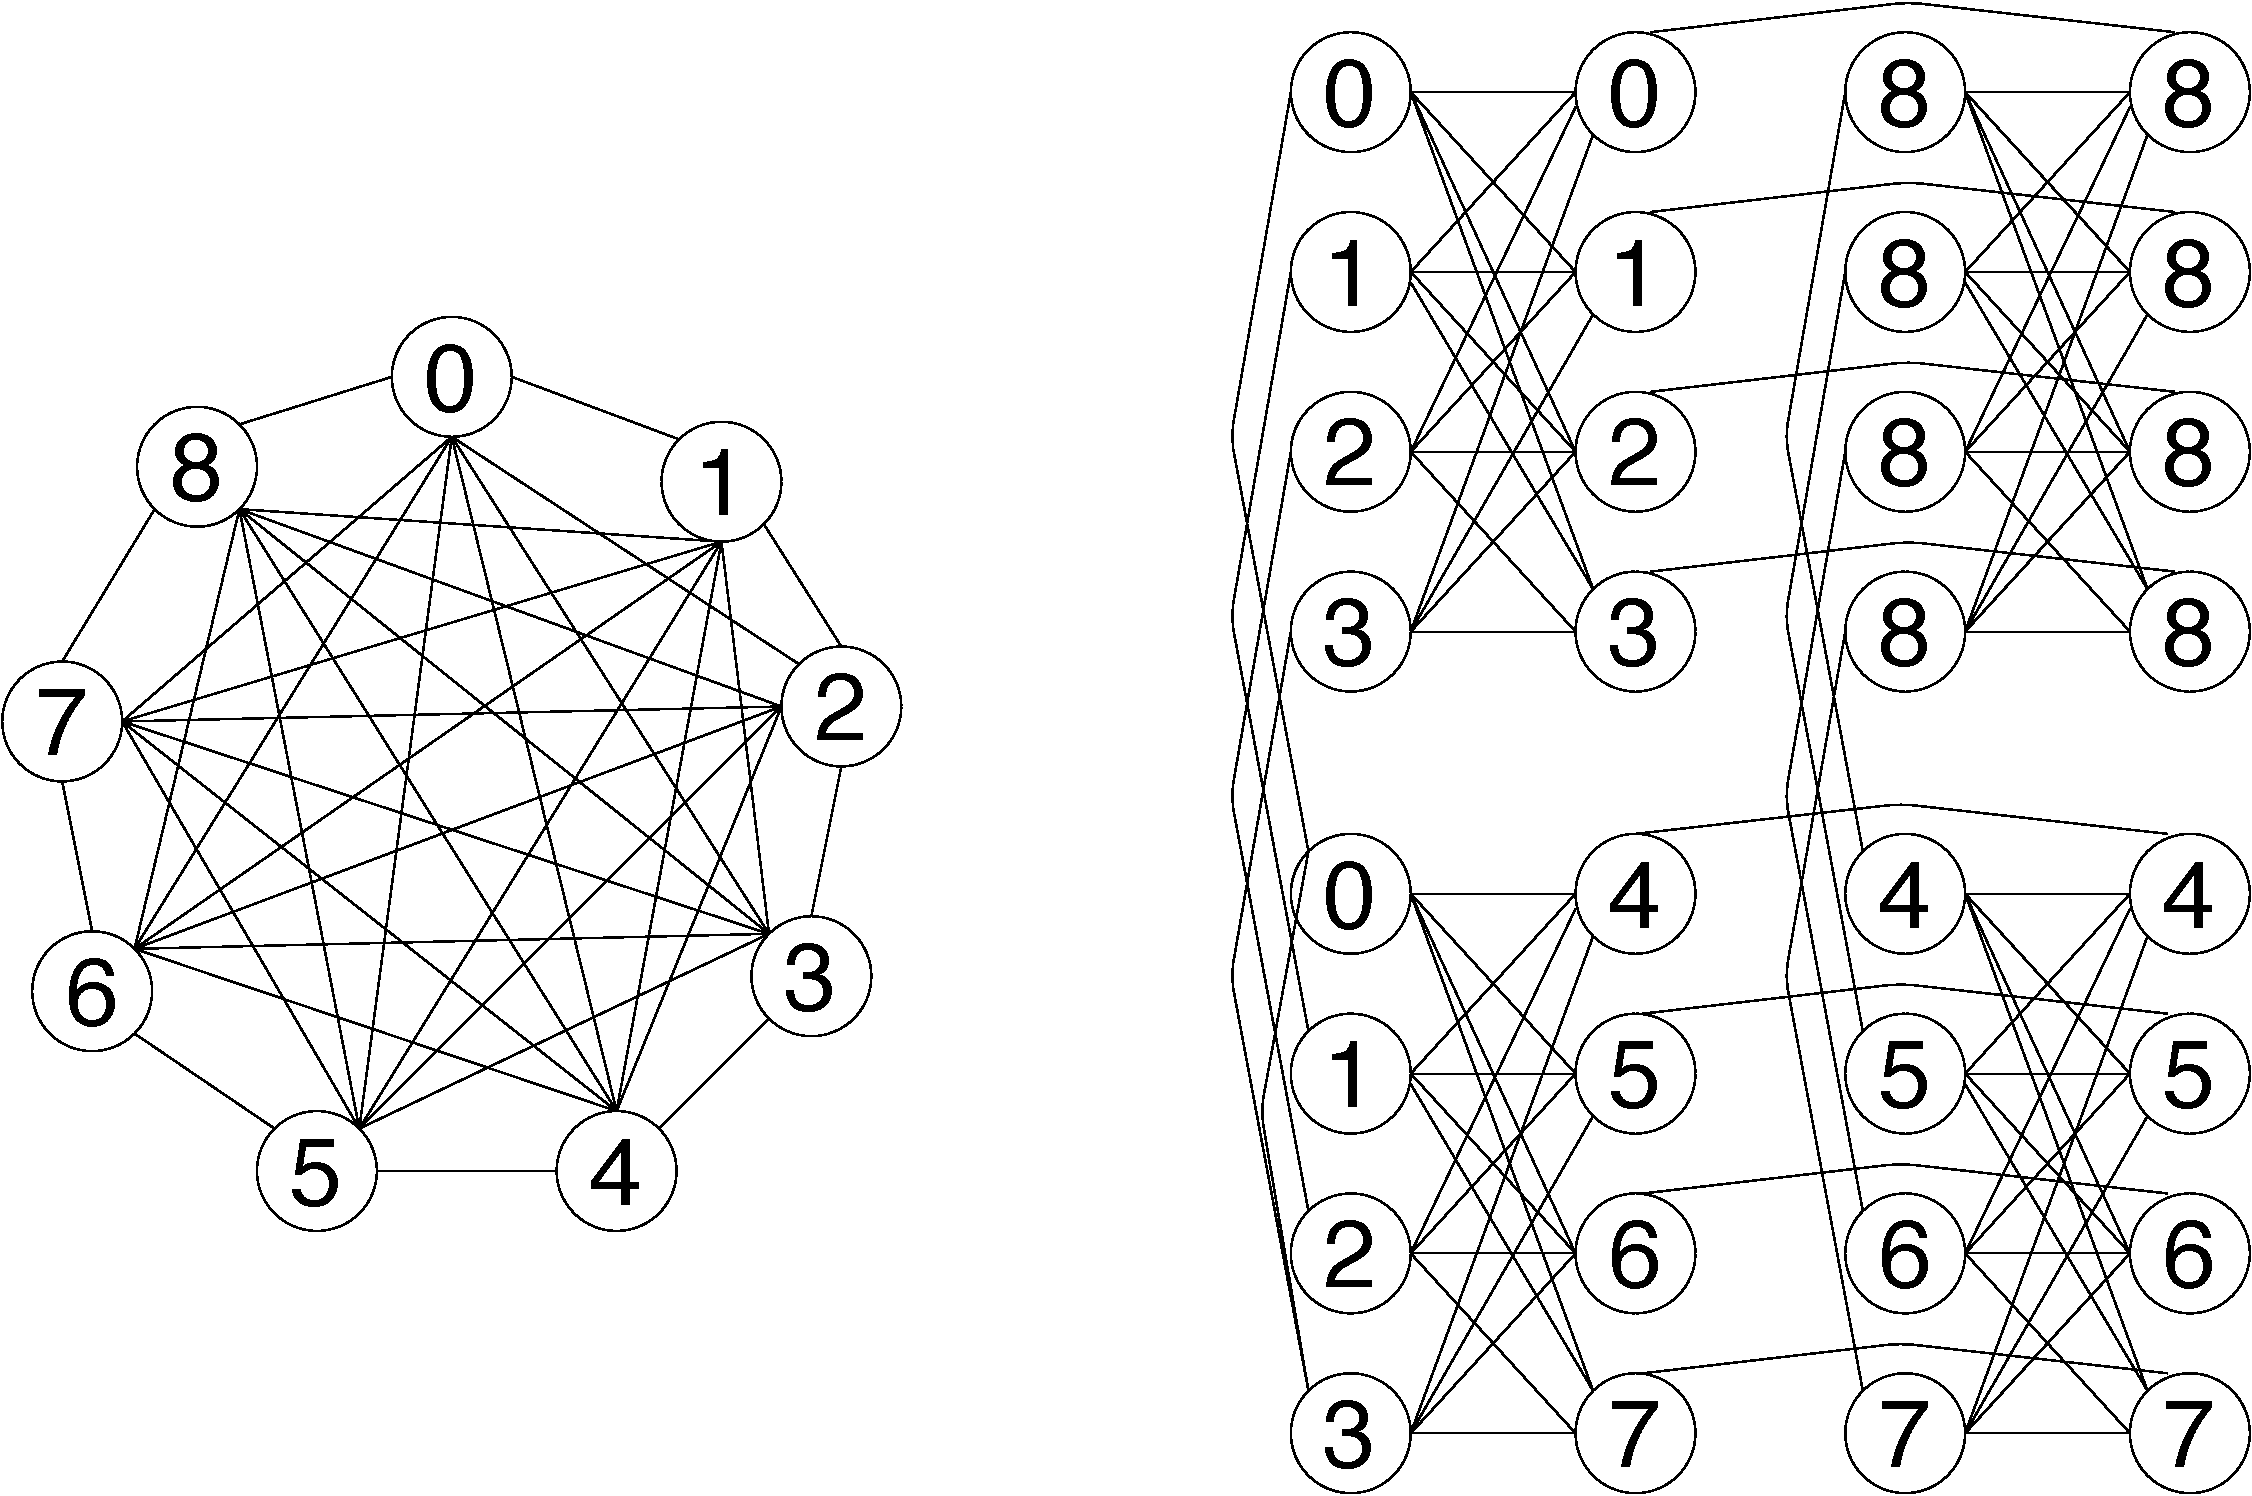
\includegraphics[width=0.5\linewidth]{img/18/complete_chimera_k9_v2.pdf}
\end{figure} 
\end{frame}

